\documentclass[12pt,]{article}
\usepackage{lmodern}
\usepackage{amssymb,amsmath}
\usepackage{ifxetex,ifluatex}
\usepackage{fixltx2e} % provides \textsubscript
\ifnum 0\ifxetex 1\fi\ifluatex 1\fi=0 % if pdftex
  \usepackage[T1]{fontenc}
  \usepackage[utf8]{inputenc}
\else % if luatex or xelatex
  \ifxetex
    \usepackage{mathspec}
  \else
    \usepackage{fontspec}
  \fi
  \defaultfontfeatures{Ligatures=TeX,Scale=MatchLowercase}
    \setmainfont[]{Times New Roman}
\fi
% use upquote if available, for straight quotes in verbatim environments
\IfFileExists{upquote.sty}{\usepackage{upquote}}{}
% use microtype if available
\IfFileExists{microtype.sty}{%
\usepackage{microtype}
\UseMicrotypeSet[protrusion]{basicmath} % disable protrusion for tt fonts
}{}
\usepackage[margin=2.54cm]{geometry}
\usepackage{hyperref}
\hypersetup{unicode=true,
            pdftitle={Predictors of Lake Level Changes in Lake Tahoe, CA},
            pdfauthor={Nikki Shintaku},
            pdfborder={0 0 0},
            breaklinks=true}
\urlstyle{same}  % don't use monospace font for urls
\usepackage{longtable,booktabs}
\usepackage{graphicx,grffile}
\makeatletter
\def\maxwidth{\ifdim\Gin@nat@width>\linewidth\linewidth\else\Gin@nat@width\fi}
\def\maxheight{\ifdim\Gin@nat@height>\textheight\textheight\else\Gin@nat@height\fi}
\makeatother
% Scale images if necessary, so that they will not overflow the page
% margins by default, and it is still possible to overwrite the defaults
% using explicit options in \includegraphics[width, height, ...]{}
\setkeys{Gin}{width=\maxwidth,height=\maxheight,keepaspectratio}
\IfFileExists{parskip.sty}{%
\usepackage{parskip}
}{% else
\setlength{\parindent}{0pt}
\setlength{\parskip}{6pt plus 2pt minus 1pt}
}
\setlength{\emergencystretch}{3em}  % prevent overfull lines
\providecommand{\tightlist}{%
  \setlength{\itemsep}{0pt}\setlength{\parskip}{0pt}}
\setcounter{secnumdepth}{5}
% Redefines (sub)paragraphs to behave more like sections
\ifx\paragraph\undefined\else
\let\oldparagraph\paragraph
\renewcommand{\paragraph}[1]{\oldparagraph{#1}\mbox{}}
\fi
\ifx\subparagraph\undefined\else
\let\oldsubparagraph\subparagraph
\renewcommand{\subparagraph}[1]{\oldsubparagraph{#1}\mbox{}}
\fi

%%% Use protect on footnotes to avoid problems with footnotes in titles
\let\rmarkdownfootnote\footnote%
\def\footnote{\protect\rmarkdownfootnote}

%%% Change title format to be more compact
\usepackage{titling}

% Create subtitle command for use in maketitle
\providecommand{\subtitle}[1]{
  \posttitle{
    \begin{center}\large#1\end{center}
    }
}

\setlength{\droptitle}{-2em}

  \title{Predictors of Lake Level Changes in Lake Tahoe, CA}
    \pretitle{\vspace{\droptitle}\centering\huge}
  \posttitle{\par}
  \subtitle{\url{https://github.com/nmshintaku/Data_Analytics_final_project}}
  \author{Nikki Shintaku}
    \preauthor{\centering\large\emph}
  \postauthor{\par}
    \date{}
    \predate{}\postdate{}
  

\begin{document}
\maketitle

\newpage
\tableofcontents 
\newpage
\listoftables 
\newpage
\listoffigures 
\newpage

\begin{figure}
\centering
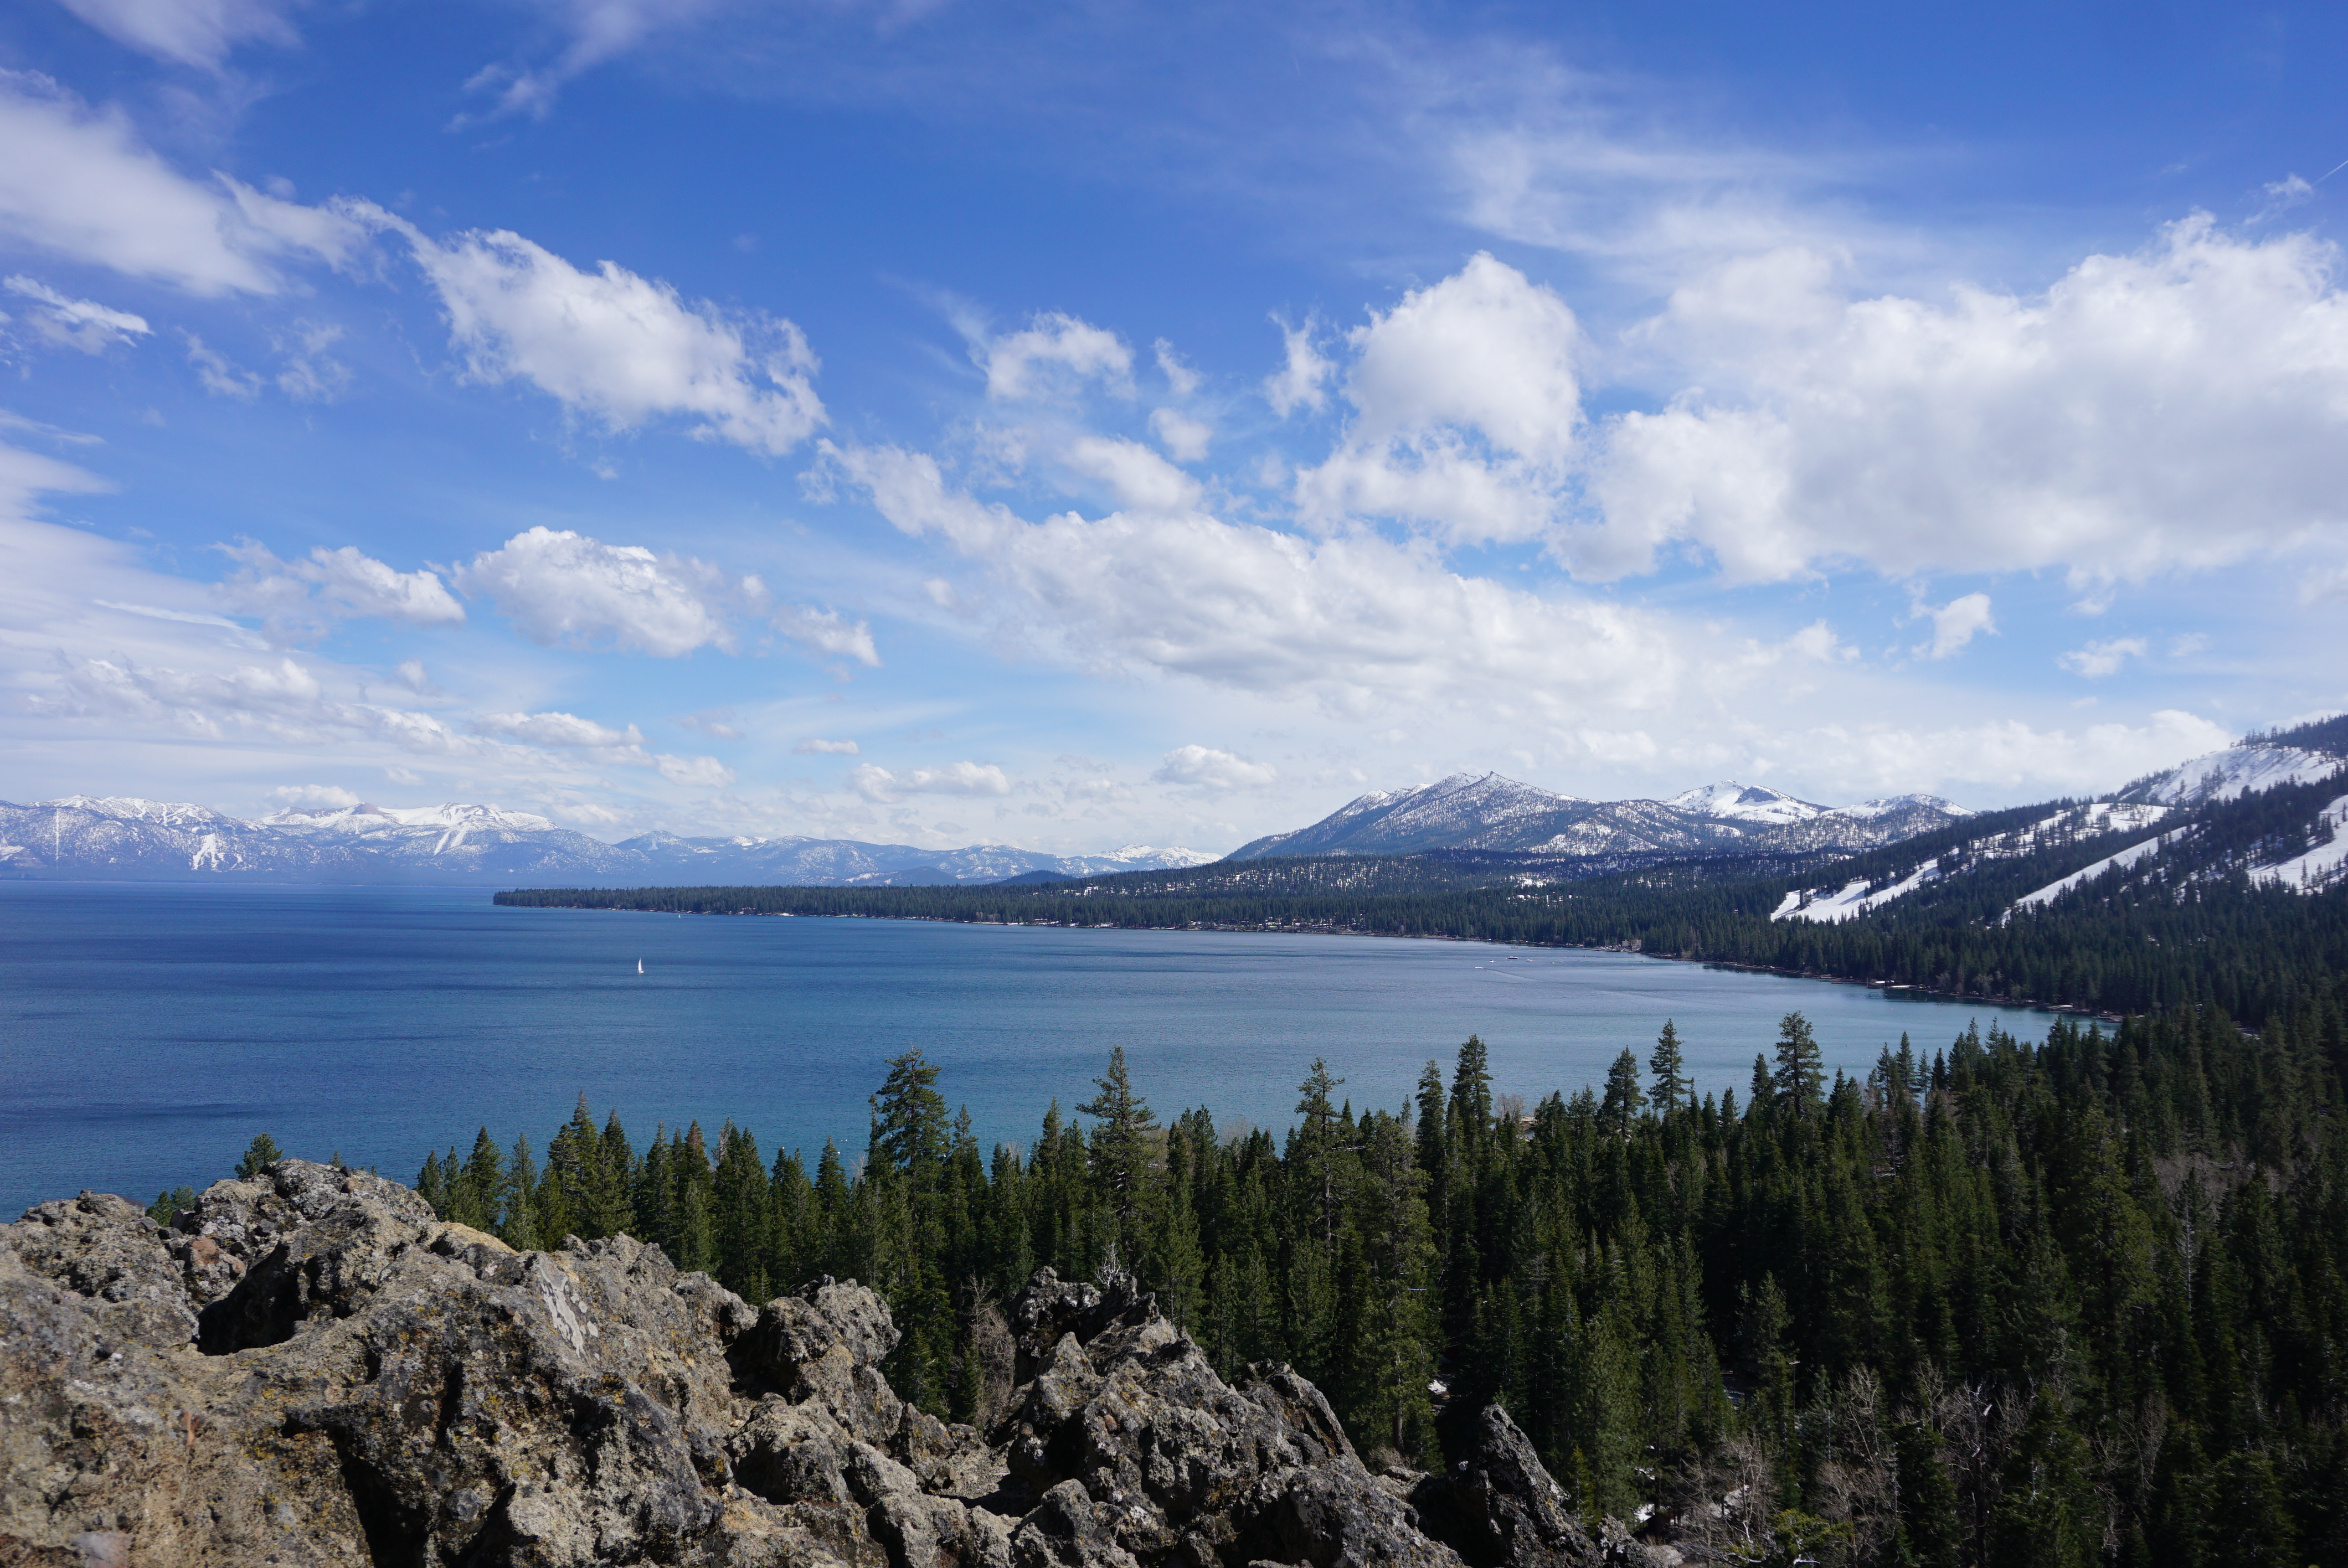
\includegraphics{Tahoe.png}
\caption{caption}
\end{figure}

\hypertarget{rationale-and-research-questions}{%
\section{Rationale and Research
Questions}\label{rationale-and-research-questions}}

Lake Tahoe measures at 6,220 feet above sea level, and is 22 miles long
and 12 miles long spanning across the California-Nevada state border.
Lake Tahoe water is 99.994\% pure contributing its legendary, beautiful
water clarity. However, Lake Tahoe is facing decline of water clarity
and health from the impacts of climate change, invasive species, and
pollution. Climate change is causing more precipitation to fall as rain
rather than snow, which leads to increase stormwater runoff carrying
sediment into Lake Tahoe. In addition, California is experiencing
extended droughts affecting amount of annual precipitation.
Inadvertently, climate change is also increasing the lake's water
temperature and affecting regional weather patterns that could change
the lake's ecosystem. Snowmelt from 63 tributaries in the watershed adds
65\% of Lake Tahoe's water, and the other 35\% falls as precipitation
directly in the lake.

Lake Tahoe's water level is controlled at the Tahoe City Dam, its only
outlet. The legal limit for water above the natural rim at that dam is
6,229.1 ft. If the lake reaches its legal limit, flooding would begin to
impact the area along with damage from erosion. With the unforeseeable
consequences of climate change and the task to keep water levels below
maximum legal limit, it is important to understand what atmospheric
factors play a role in Lake Tahoe's water level.

This analysis investigates the trends in Lake Tahoe's water level
accross the time period 1957 - 2019, and the possible drivers of lake
level through the research questions:

\begin{enumerate}
\def\labelenumi{\arabic{enumi}.}
\item
  How does lake level in Lake Tahoe change over the years?
\item
  What are significant atmospheric predictors of lake level in Lake
  Tahoe?
\end{enumerate}

The gage station site for measuring lake water level (or gage height) is
located in Tahoe City, CA where the dam is controlled, and the data was
downloaded from USGS. Subsequent atmospheric data include precipitation,
snow fall, snow depth, average daily temperature, maximum daily
temperature, and minimum daily temperature downloaded from NOAA and
subsetted to the Tahoe City, CA station to be as accurate as possible
for data collection location.

\emph{Fun Fact: If you were to pour Lake Tahoe out onto an area the size
of California, the water would still be 14 inches deep.}

\newpage

\hypertarget{dataset-information}{%
\section{Dataset Information}\label{dataset-information}}

\hypertarget{usgs-gage-height-data}{%
\subsection{USGS Gage Height Data}\label{usgs-gage-height-data}}

The data for lake level was downloaded from USGS Water-Quality Data for
the Nation website at \url{https://waterdata.usgs.gov/nwis/qw}. The
dataset contains daily gage height measurements in feet from January
1920 - December 2019 from one station (Site \#103370000) in Tahoe City,
CA. USGS reports that gage height is measured from the recorded lake
elevation of 6,220 ft as the zero basline. Gage height measurement +
current lake elevation (6,220 ft) will give the actual lake level from
sea level.

This dataset was relatively easy to wrangle; unneccesary columns were
dropped, leaving only date and gage height. There was a time period from
January 1920 - April 1920 with gage height measurements, and then no
measurements until October 1, 1957 so a decision was made to remove the
3 months of data in 1920 because the gap between 1920 and 1957 is too
large to interpolate daily measurements. In addition, the three months
of data is too short of a time period to do a time series analysis.
After that wranging, there were 3 gage height NAs so these were linearly
interpolated to create a complete dataset.

\begin{longtable}[]{@{}ll@{}}
\caption{\label{tab:table} USGS Gage Height Data Summary}\tabularnewline
\toprule
Data & Summary\tabularnewline
\midrule
\endfirsthead
\toprule
Data & Summary\tabularnewline
\midrule
\endhead
Total Number of Samples & 22,737\tabularnewline
Start Date & 1957-10-01\tabularnewline
End Date & 2019-12-31\tabularnewline
Gage Height Mean (ft) & 5.86\tabularnewline
Gage Height Median (ft) & 6.32\tabularnewline
Gage Height Min (ft) & 0.26\tabularnewline
Gage Height Max (ft) & 9.40\tabularnewline
\bottomrule
\end{longtable}

\hypertarget{noaa-climate-data}{%
\subsection{NOAA Climate Data}\label{noaa-climate-data}}

The atmospheric data was downloaded from NOAA National Centers for
Environmental Information at \url{https://www.ncdc.noaa.gov/cdo-web/}.
This dataset contains daily measurements for precipitation, snow fall,
snow depth, average daily temperature, maximum daily temperature, and
minimum daily temperature beginning from September 13, 1903 - March 30,
2020 from 5 different stations within the zip code of 96145 (for Tahoe
City, CA). Precipitation, snowfall, and snow depth are measured in
inches, and temperatures are all measured in fahrenheit.

With such a large time period for this dataset, there is a lot of NAs
and an uneven amount of measurements across the stations. To be as
accurate as possible for location of both the gage height station and
climate station, the station named ``TAHOE CITY, CA US'' was filterd out
to be used in this analysis. The data for the Tahoe City station ranges
from September 13, 1903 - March 30, 2020 so the dates were filtered to
match the same time period as the gage height measurements from October
1, 1957 - December 31, 2019. From here, presence of NAs were checked,
and the entire column for average daily temperature was NAs so that
column was deleted entirely. The rest of the data with NAs were linearly
interpolated to create a complete dataset.

\begin{longtable}[]{@{}llllll@{}}
\caption{\label{tab:table} NOAA Tahoe City Climate Data
Summary}\tabularnewline
\toprule
Variable & Date & Mean & Median & Min & Max\tabularnewline
\midrule
\endfirsthead
\toprule
Variable & Date & Mean & Median & Min & Max\tabularnewline
\midrule
\endhead
Start Date & 1957-10-01 & - & - & - & -\tabularnewline
End Date & 2019-12-31 & - & - & - & -\tabularnewline
Precipitation (in) & - & 0.09 & 0 & 0 & 6.77\tabularnewline
Snow Fall (in) & - & 0.49 & 0 & 0 & 42\tabularnewline
Snow Depth (in) & - & 7.74 & 0 & 0 & 120\tabularnewline
Daily Temp Max (F) & - & 56.82 & 55 & 11 & 94\tabularnewline
Daily Temp Min (F) & - & 31.35 & 31 & -16 & 79\tabularnewline
\bottomrule
\end{longtable}

Lastly, the USGS processed data and the NOAA Tahoe City climate
processed data were joined together by date to create a large dataset
containing gage height and climate data together. For data explorataion
and visualization purposes, temperature in celsisus was calculated for
minimum and maximum daily temperatures.

\newpage

\hypertarget{exploratory-analysis}{%
\section{Exploratory Analysis}\label{exploratory-analysis}}

\newpage

\hypertarget{analysis}{%
\section{Analysis}\label{analysis}}

\hypertarget{question-1-insert-specific-question-here-and-add-additional-subsections-for-additional-questions-below-if-needed}{%
\subsection{Question 1: \textless{}insert specific question here and add
additional subsections for additional questions below, if
needed\textgreater{}}\label{question-1-insert-specific-question-here-and-add-additional-subsections-for-additional-questions-below-if-needed}}

\hypertarget{question-2}{%
\subsection{Question 2:}\label{question-2}}

\newpage

\hypertarget{summary-and-conclusions}{%
\section{Summary and Conclusions}\label{summary-and-conclusions}}

\newpage

\hypertarget{references}{%
\section{References}\label{references}}

\textless{}add references here if relevant, otherwise delete this
section\textgreater{}


\end{document}
